\documentclass{article}
\usepackage{graphicx} % Required for inserting images
\usepackage[margin=1in]{geometry}
\usepackage[T1]{fontenc}
\usepackage{lmodern}
\usepackage{booktabs}   % nicer tables
\usepackage{array}      % ragged-right column in the table
\usepackage{float}      % [H] keeps figures where they are written
\usepackage{caption}
\usepackage{amsmath}
\usepackage{xcolor}
\usepackage[round]{natbib}  % author-year citations: \citep{key}
\usepackage[colorlinks=true,linkcolor=blue,citecolor=blue,urlcolor=blue]{hyperref}

\captionsetup{font=small,labelfont=bf}
% Gene names are always in italics
\newcommand{\gene}[1]{\textit{#1}}

\title{HSE103_FinalProject}
\author{Zhiying(Winnie) Chen}
\date{November 2026}

\begin{document}

\maketitle
% =======================================
\section{Methods}

\subsection{Data source and initial sample size}
The data come from a nested case-control study within the Vitamin D Antenatal Asthma
Reduction Trial (VDAART) \citep{Mirzakhani2016}. Gene expression was measured in whole
blood collected at 10 to 18 weeks of pregnancy from 157 women, 47 who later developed
preeclampsia and 110 controls \citep{Mirzakhani2016}, and the data are available in the
NCBI Gene Expression Omnibus as GSE85307 \citep{GSE85307}. The initial sample size was
therefore $n = 157$ women. The files provided for this project contained 500 genes (of
the 750 genes listed in the annotation file) and, for each woman, maternal age, BMI,
vitamin D level (ng/mL), asthma status, gestational age at sample collection and at
delivery, microarray batch and pregnancy condition (Normal or Preeclampsia).

\subsection{Final sample size}
The final sample size was $n = 157$ (110 Normal and 47 Preeclampsia), so no women were removed. There were no missing values in the covariates or the expression data that were used. Five women had a BMI below 18.5~kg/m$^2$, but they were too few for their own group and were kept in the $<$25 BMI Group. One woman had a vitamin D level of about 80~ng/mL, much higher than the others (Figure~\ref{fig:final_scatter}); this value was kept because it is a measure value with no sign of a measurement error, but it has a large influence on the fitted line, so the vitamin D results should be read this in mind. Expression values were used as provided, without further normalization or transformation.

\subsection{Analyses}
\paragraph{Covariates.}BMI was grouped into $<$25, 25-30 and $\geq$30~kg/m$^2$. For the summary table, continuous variables were described by the median and terquartile range (IQR) when their histograms were skewed (vitamin D and gestational age at delivery) and by the mean and standard deviation (SD) when they were roughly symmetric (maternal age); BMI group is reported as the number and percentage of women.
The table is stratified by pregnancy condition.

\paragraph{Plots for one gene.} For \gene{GNLY}, I made a histogram of expression, a scatter plot of expression against maternal vitamin D with a linear fit and the Pearson correlation, and boxplots of expression by BMI group and pregnancy condition with every woman shown as a point.

\paragraph{Heatmap.}The 10 genes with the highest variance in expression across the 157 women were selected. Each gene was scaled to a mean of 0 and a standard deviation of 1 across women, and both genes and women were clustered by hierarchical clustering (Euclidean distance and complete linkage, the defaults of the \texttt{pheatmap} package). Tracking bars show pregnancy condition and BMI group.

\paragraph{Volcano Plot.} Women were split at 30~ng/mL, the cut point for vitamin D sufficiency used in the original stydy \citep{Mirzakhani2016}: vitamin D $\geq$30~ng/mL ($n=38$) and $<$30~ng/mL ($n=119$). For each of the 500 genes, the two groups were compared with a Welch $t$ test. The $x$-axis of the volcano plot is the diffenrence in mean expressin ($\geq$30 minus $<$30) and the $y$-axis is $-\log_{10}$ of the $p$ value. Genes with $p < 0.05$ are colored as high (Up) or lower (Down) in the $\geq$30 group, and the other genes are labeled NotSig. Because 500 tests were run, the Bonferroni cutoff ($0.05/500 = 0.0001$) is also shown. No analysis was adjusted for other covariates or for the microarray batch.

\subsection{Software}
All analyses were done in R version 4.6.1 \citep{Rbase} with the tidyverse version 2.0.0 \citep{tidyverse}, including ggplot2 version 4.0.3 \citep{ggplot2}, the ggpubr package version 1.0.0 \citep{ggpubr} and the pheatmap version 1.0.13 \citep{pheatmap}. The report was typest in \LaTeX{} using Overleaf.

\subsection{Code availability}
The code, data files and figures for all submissions of this project are in the GitHub repository \url{https://github.com/winnie-chan1014/HSE103-final-project}.

%========================================================
\section{Results}

\subsection{Summary statistics}
Table~\ref{tab:summary} describes the 157 women. Women who developed preeclampsia
had a lower median vitamin D level than Normal women (17.70 vs.\ 21.80~ng/mL) and
were more often in the BMI $\geq$30 group (55.3\% vs.\ 28.2\%)
(Table~\ref{tab:summary}). These are descriptive comparisons without a statistical
test, and because cases and controls were sampled in a fixed ratio, the percentages do
not show the risk of preeclampsia.

\begin{table}[H]
\centering
\caption{Summary Statistics}
\label{tab:summary}
\begin{tabular}{llll}
Variable                                              & Overall (n = 157)        & Normal (n = 110)         & Preeclampsia (n = 47)    \\
Maternal vitamin D (ng/mL), median {[}IQR{]}          & 20.40 {[}13.40, 29.50{]} & 21.80 {[}13.85, 32.08{]} & 17.70 {[}12.55, 27.40{]} \\
Maternal age (years), mean (SD)                       & 26.38 (5.04)             & 26.63 (5.08)             & 25.78 (4.95)             \\
Gestational age at delivery (weeks), median {[}IQR{]} & 39.29 {[}38.14, 40.00{]} & 39.29 {[}38.57, 40.00{]} & 39.14 {[}36.93, 40.07{]} \\
BMI group (kg/m²), n (\%)                             &                          &                          &                          \\
\textless{}25                                         & 53 (33.8)                & 40 (36.4)                & 13 (27.7)                \\
25-30                                                 & 47 (29.9)                & 39 (35.5)                & 8 (17.0)                 \\
$\geq$30                                              & 57 (36.3)                & 31 (28.2)                & 26 (55.3)               
\end{tabular}
\end{table}

\subsection{Gene expression and covariates (\gene{GNLY})}
\gene{GNLY} expression had a single main peak, with values from 8.80 to 11.23
(Figure~\ref{fig:hist}). \gene{GNLY} expression decreased as maternal vitamin D
increased ($r = -0.28$, $p < 0.001$; Figure~\ref{fig:scatter}). \gene{GNLY} expression
was highest in the BMI $\geq$30 group (median 10.31 in Normal and 10.22 in
Preeclampsia women, compared with 9.94 to 10.02 in the other groups), and it was
similar between Normal and Preeclampsia women within each BMI group
(Figure~\ref{fig:box}). No formal test was done for the BMI and pregnancy condition
comparisons, and the Preeclampsia group with BMI 25--30 had only 8 women.

\begin{figure}[H]
\centering
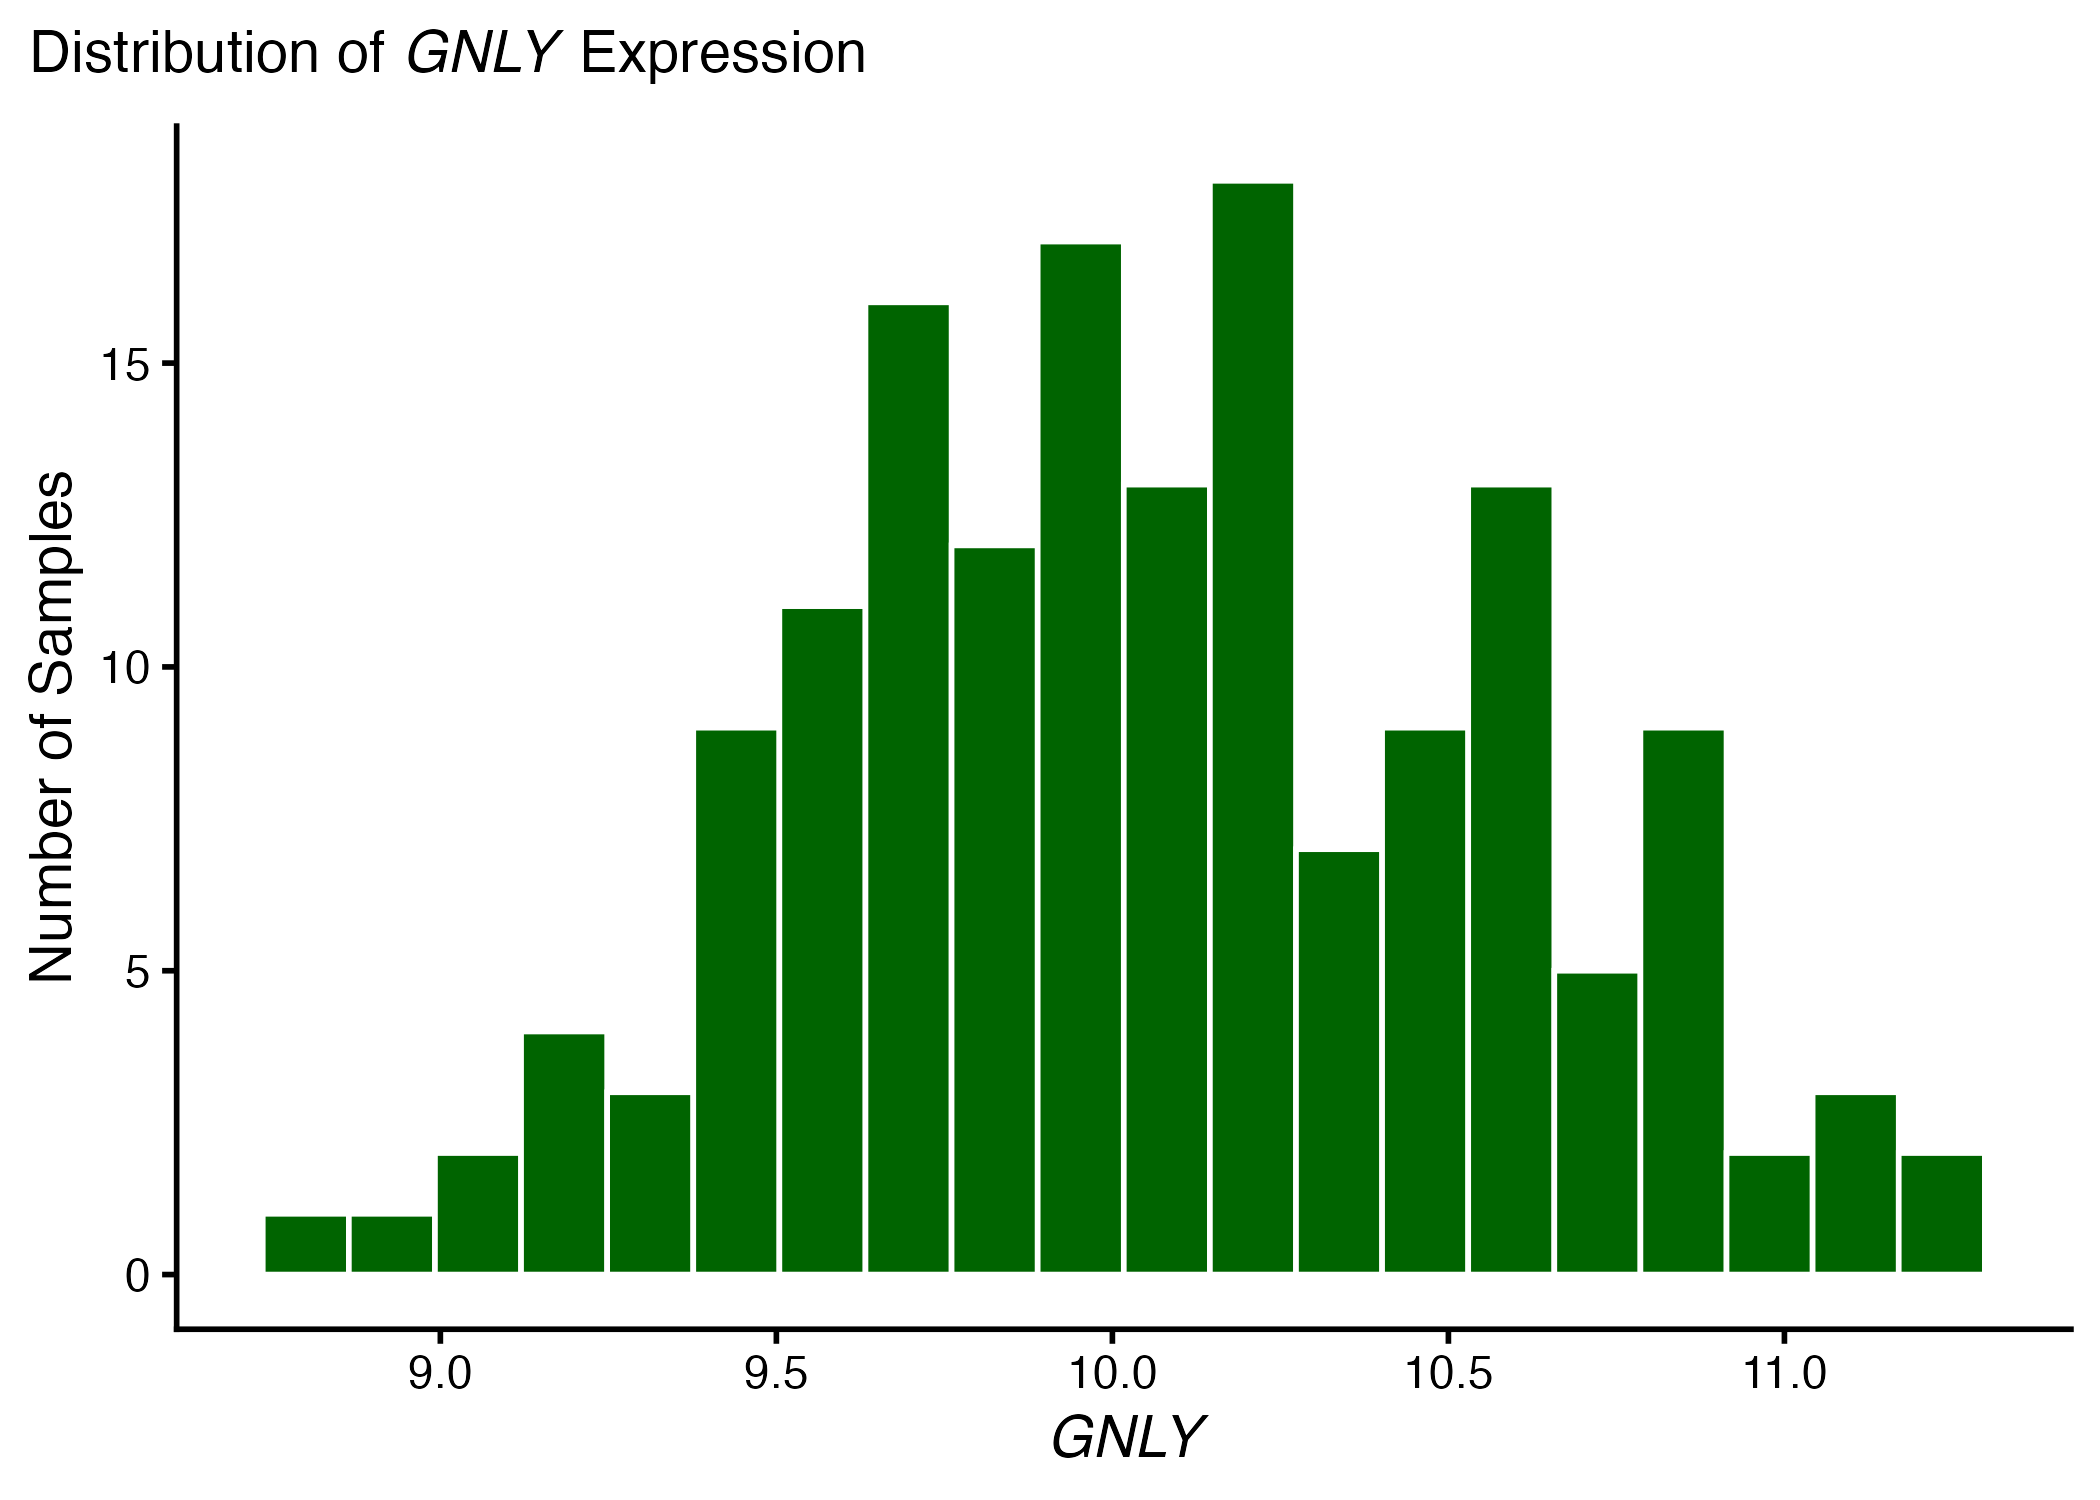
\includegraphics[width=0.8\textwidth]{final_histogram.png}
\caption{Distribution of \gene{GNLY} expression in all 157 women. Each bar is one of
20 equal-width bins, and the $y$-axis is the number of women.}
\label{fig:hist}
\end{figure}

\begin{figure}[H]
\centering
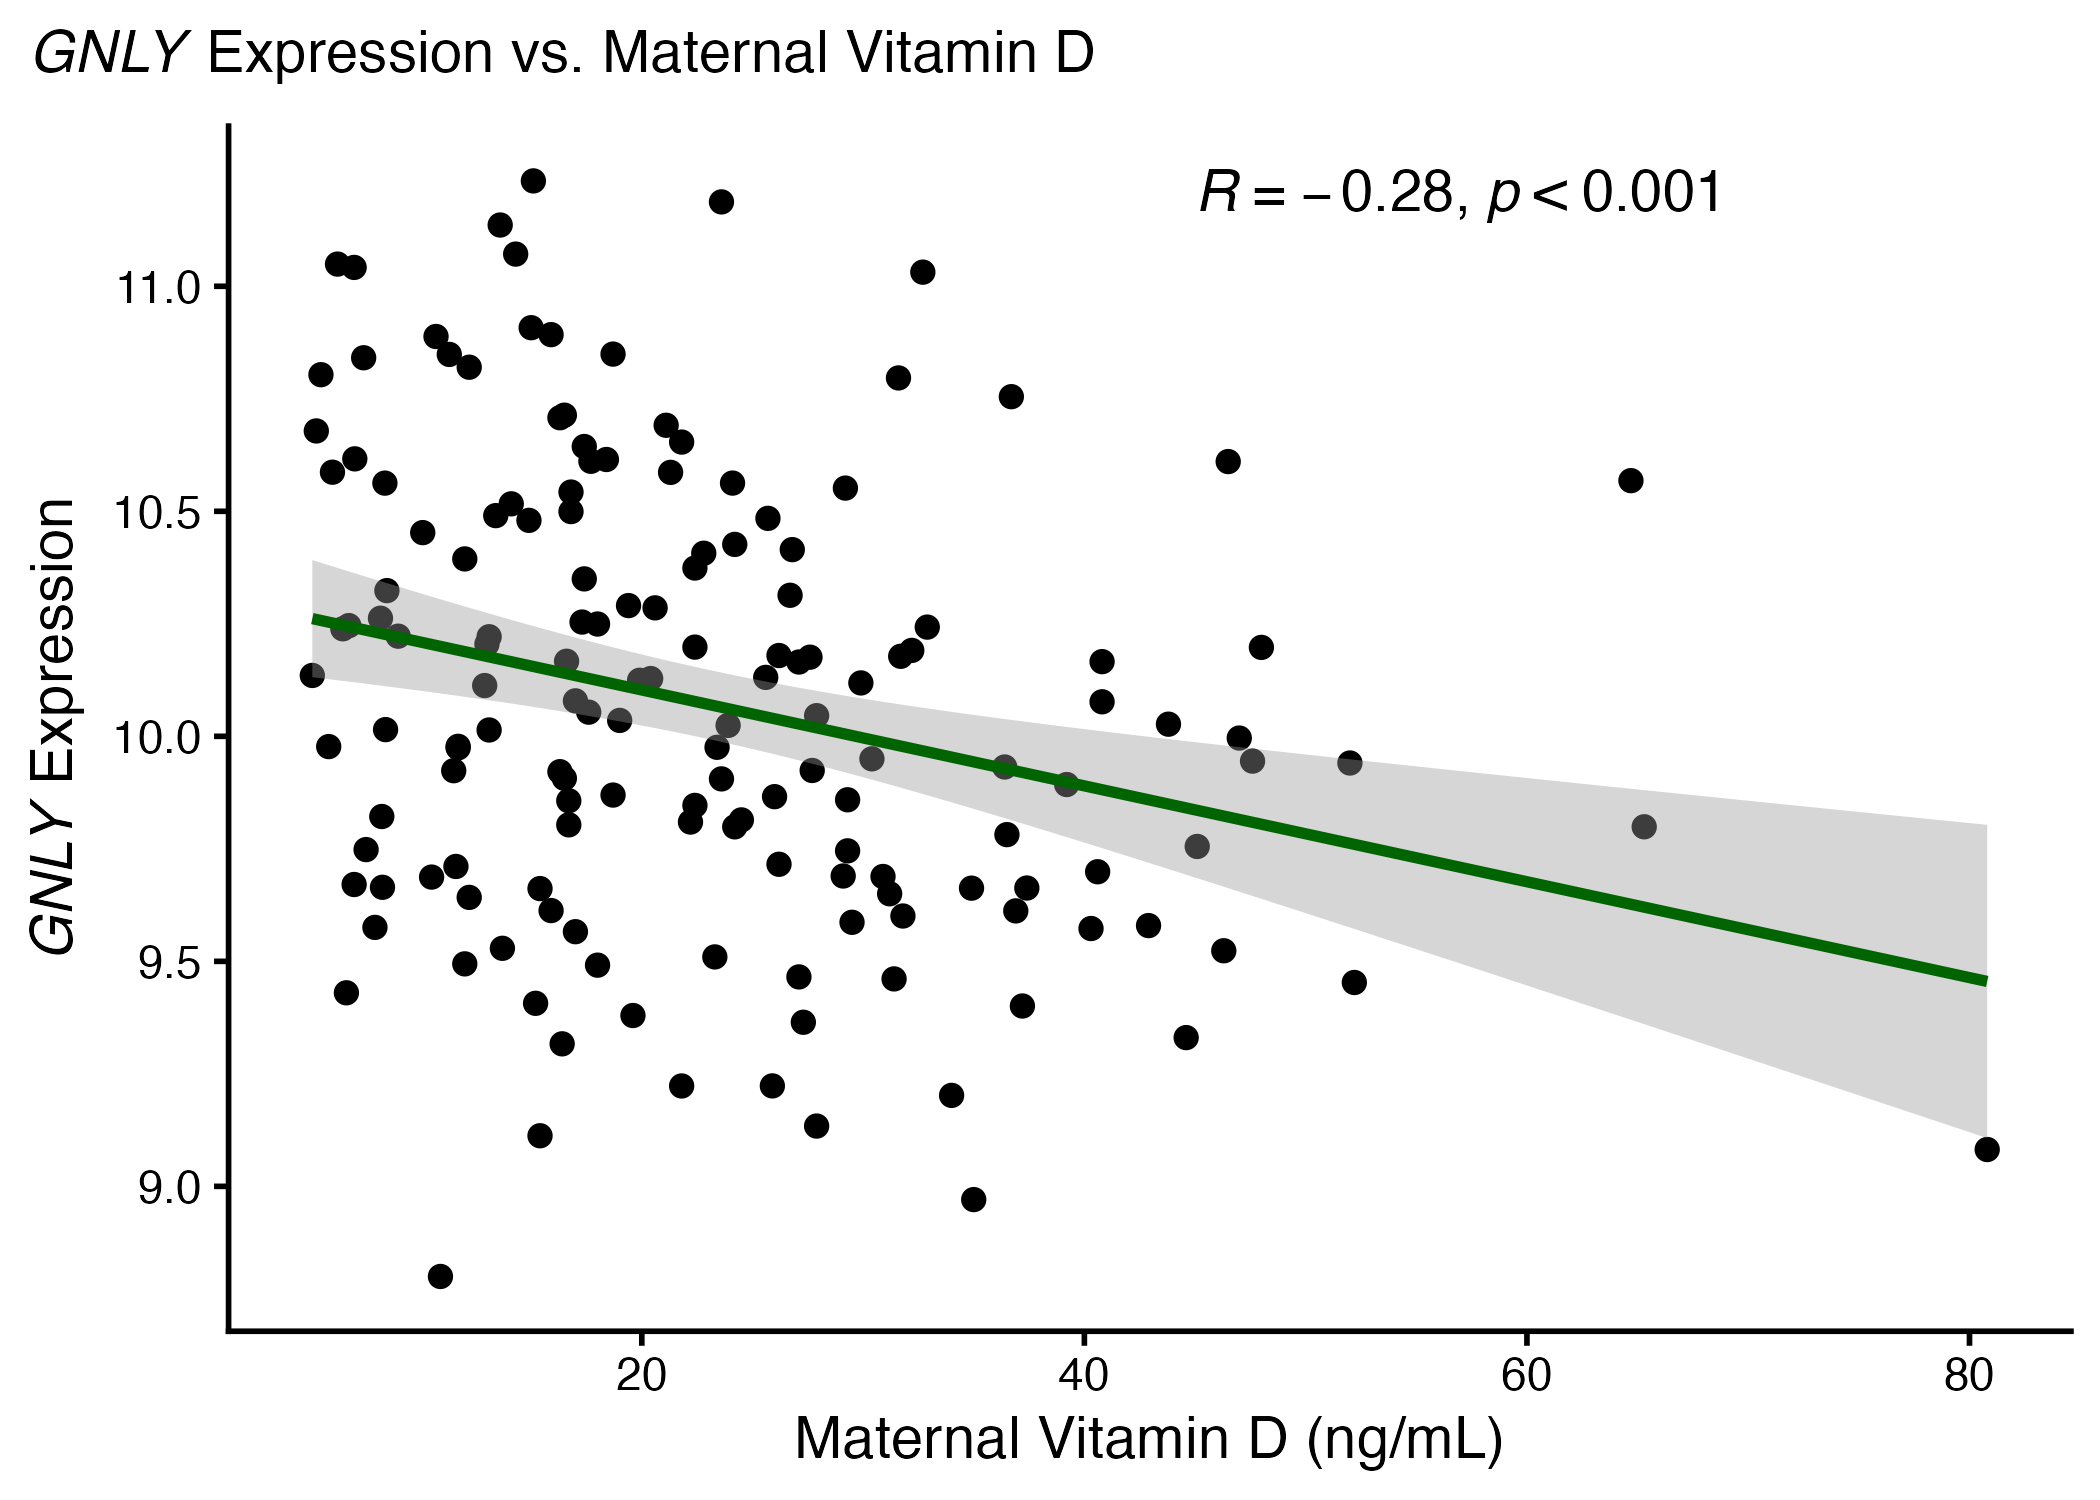
\includegraphics[width=0.8\textwidth]{final_scatter.png}
\caption{\gene{GNLY} expression against maternal vitamin D. Each point is one woman
($n = 157$). The line is the linear fit and the shaded band is its 95\% confidence
interval. $R$ and $p$ are from a Pearson correlation.}
\label{fig:scatter}
\end{figure}

\begin{figure}[H]
\centering
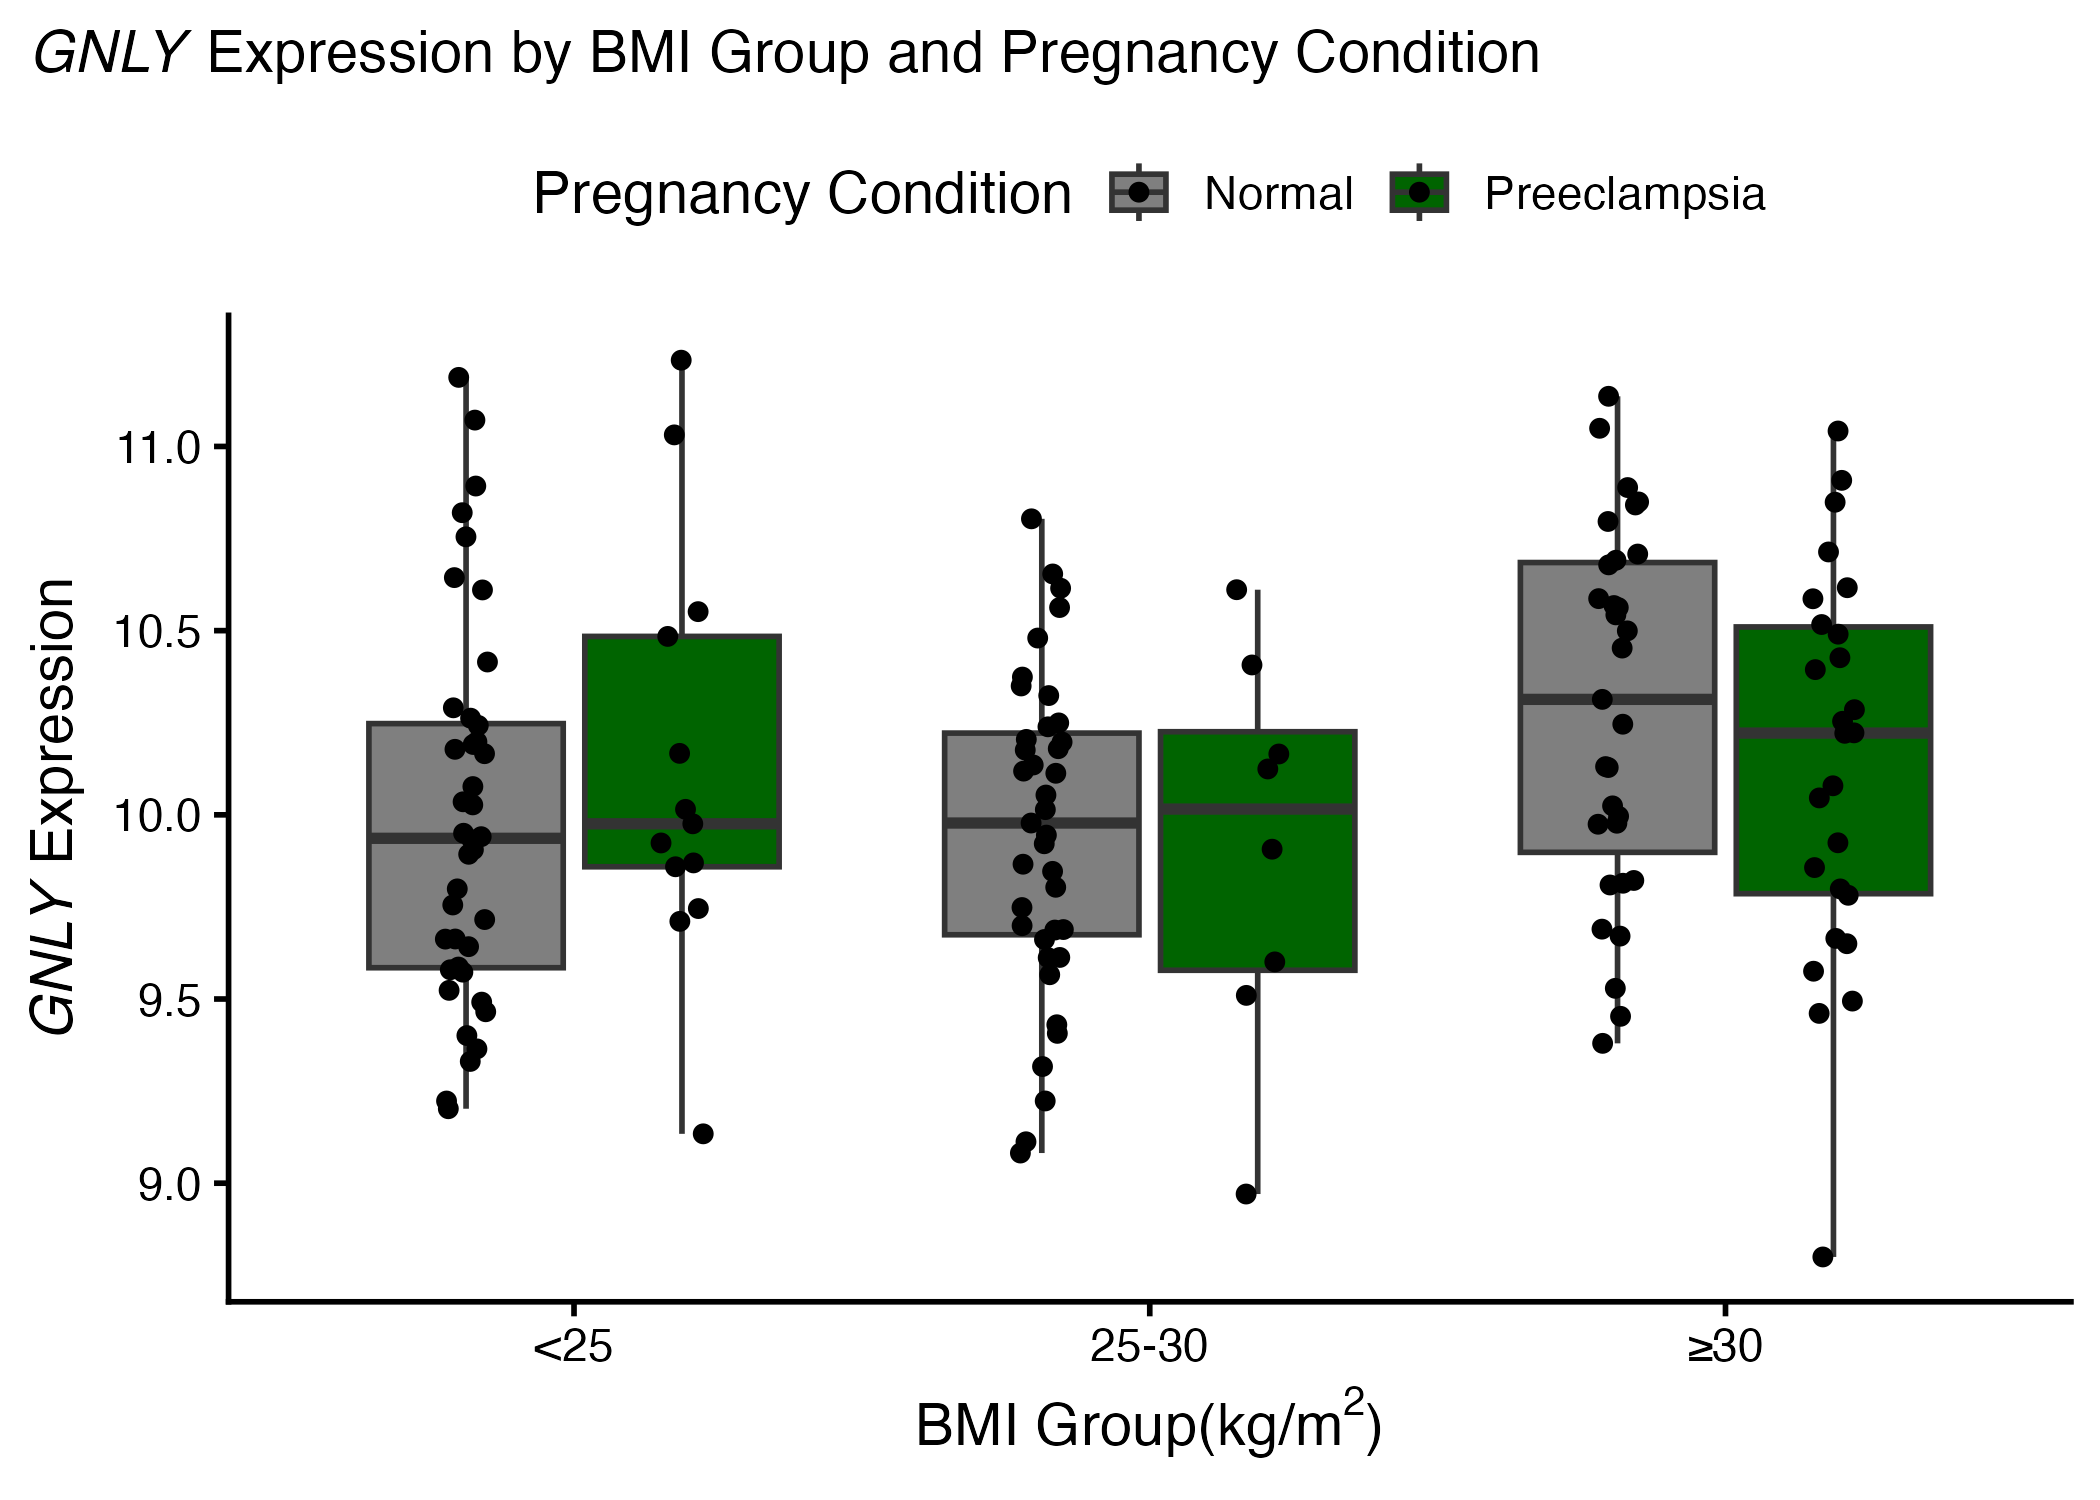
\includegraphics[width=0.8\textwidth]{final_boxplot.png}
\caption{\gene{GNLY} expression by BMI group and pregnancy condition. The line inside
each box is the median, the box is the interquartile range, the whiskers extend to 1.5
times the interquartile range, and each point is one woman. The numbers under each
BMI group are the numbers of Normal / Preeclampsia women.}
\label{fig:box}
\end{figure}

\subsection{Heatmap of the most variable genes}
The 10 most variable genes were \gene{CEACAM6}, \gene{CLIC2}, \gene{RUNDC3A},
\gene{SLC1A5}, \gene{TGM2}, \gene{CAPZA2}, \gene{ZNF594}, \gene{ZBTB41},
\gene{UTS2} and \gene{TMEM176B}. The genes formed co-expression groups; for example,
\gene{CAPZA2}, \gene{ZNF594} and \gene{ZBTB41} clustered together
(Figure~\ref{fig:heat}). In contrast, the women did not separate into groups by
pregnancy condition or BMI group, because both tracking bars are mixed across the
sample dendrogram (Figure~\ref{fig:heat}).

\begin{figure}[H]
\centering
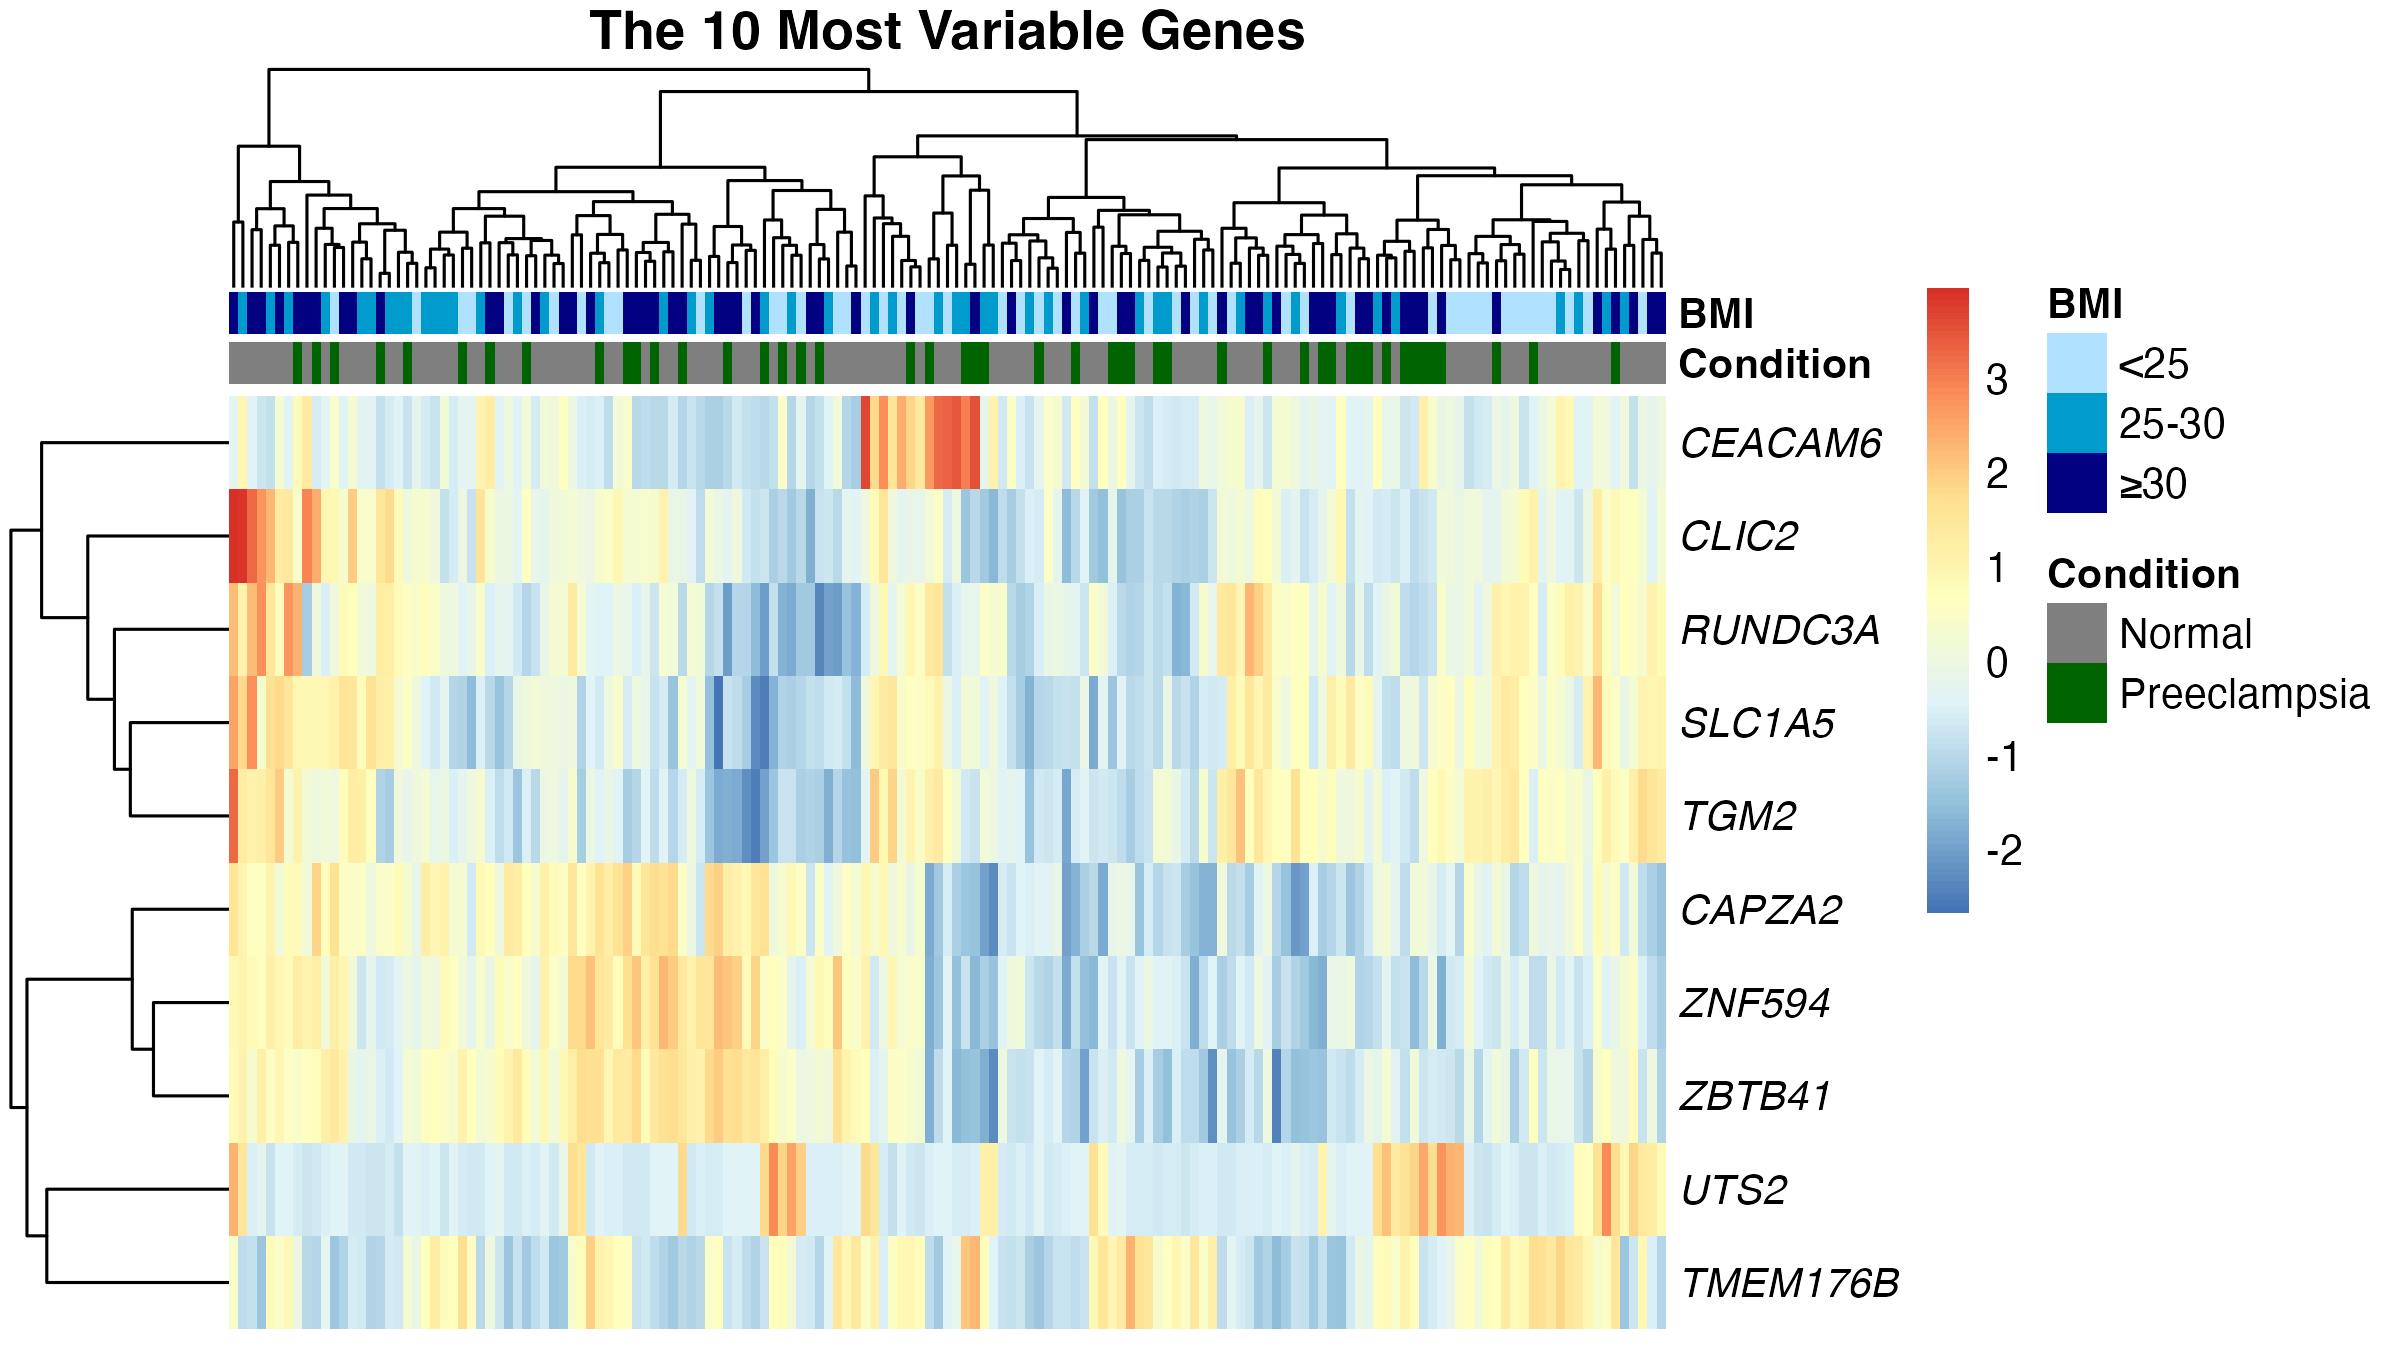
\includegraphics[width=\textwidth]{final_heatmap.png}
\caption{Heatmap of the 10 genes with the highest variance in expression. Columns are
the 157 women and rows are genes, scaled to a mean of 0 and a standard deviation of 1
within each gene (red is higher and blue is lower). Genes and women are clustered by
hierarchical clustering (Euclidean distance, complete linkage). The tracking bars above
the heatmap show BMI group and pregnancy condition.}
\label{fig:heat}
\end{figure}

\subsection{Association of every gene with Vitamin D}
Of the 500 genes, 117 had $p < 0.05$ when comparing women with vitamin D
$\geq$30~ng/mL with women below 30~ng/mL: 70 were higher (Up) and 47 were lower (Down)
in the $\geq$30 group, and 383 were not significant (NotSig) (Figure~\ref{fig:volcano}).
Fifteen genes passed the Bonferroni cutoff, 14 higher and 1 lower in the $\geq$30
group (Figure~\ref{fig:volcano}). I named \gene{GNLY}, \gene{LYN} and \gene{IL26} on
the plot because they are the genes from my earlier submissions (\gene{GNLY} in
Submission 1, and \gene{LYN} and \gene{IL26} added in Submission 2), so the plot shows
where they fall among all 500 genes. Their positions agree with my earlier analysis of
vitamin D as a continuous variable. \gene{GNLY} was lower in women with vitamin D
$\geq$30 ($p = 0.004$), as it decreased with vitamin D before ($r = -0.28$).
\gene{LYN} was higher and passed the Bonferroni cutoff ($p < 0.001$), as it increased
with vitamin D before ($r = 0.39$). \gene{IL26} was only weakly lower ($p = 0.040$),
in line with its weak negative correlation before ($r = -0.11$, $p = 0.158$); only
\gene{LYN} passed the Bonferroni cutoff (Figure~\ref{fig:volcano}).

\begin{figure}[H]
\centering
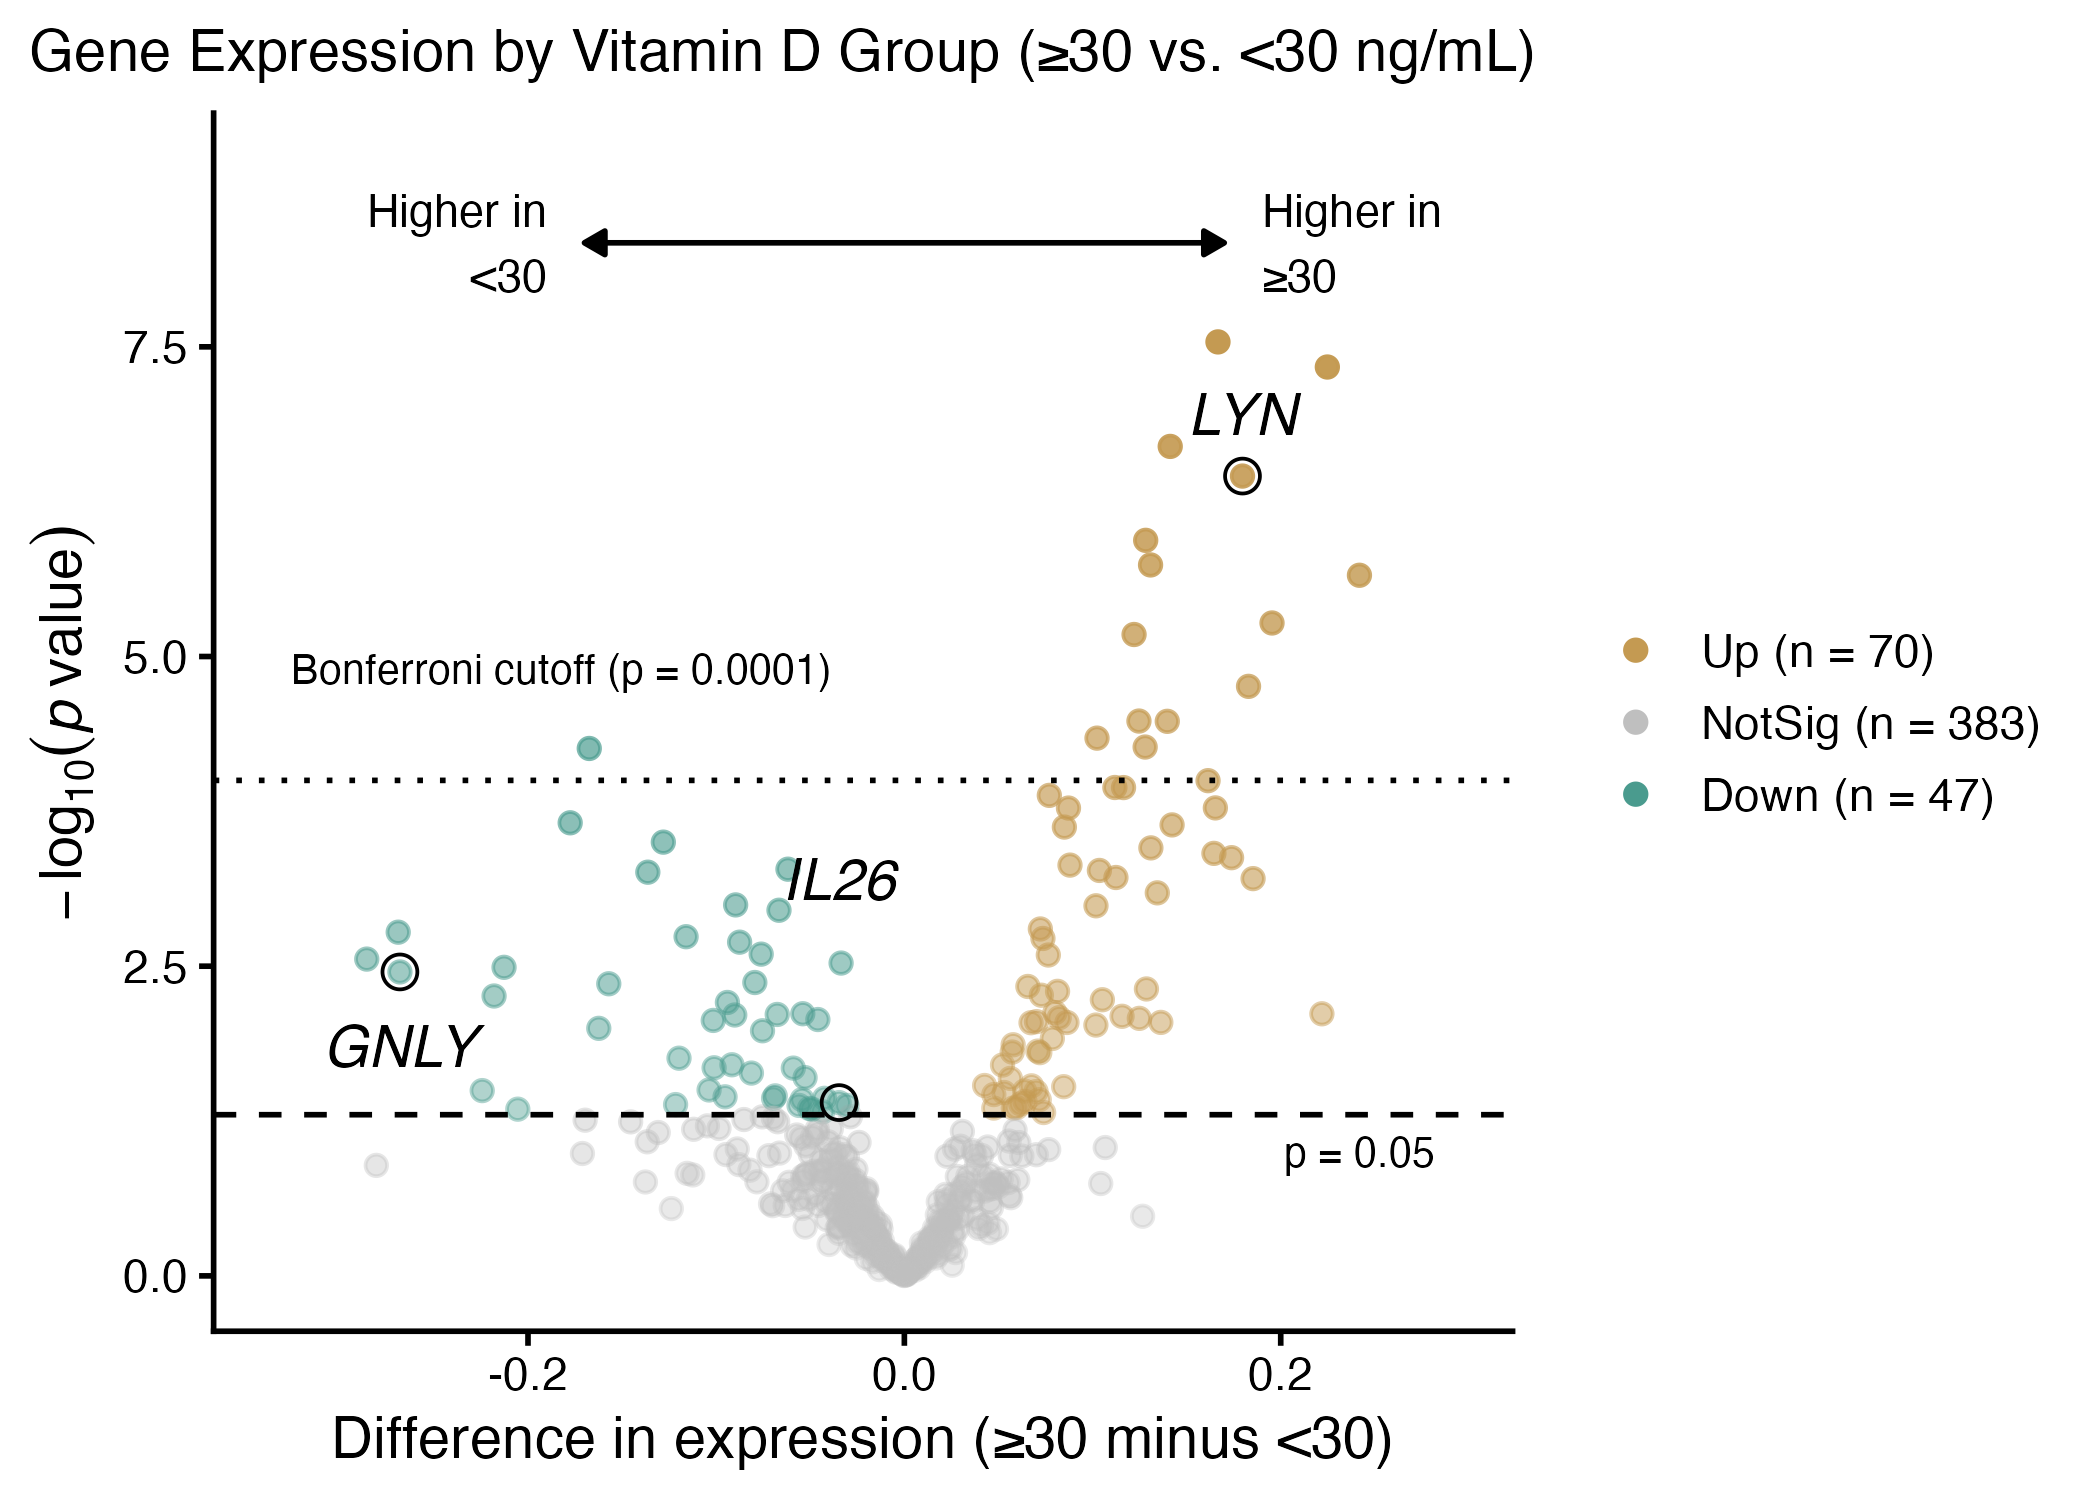
\includegraphics[width=0.9\textwidth]{final_volcano.png}
\caption{Volcano plot of the difference in gene expression between women with
vitamin D $\geq$30 and $<$30~ng/mL. Each point is one of the 500 genes. The $x$-axis is
the difference in mean expression ($\geq$30 minus $<$30) and the $y$-axis is
$-\log_{10}$ of the Welch $t$ test $p$ value. Genes with $p < 0.05$ are colored: Up is
higher and Down is lower in the $\geq$30 group, and NotSig is $p \geq 0.05$; darker
points have smaller $p$ values. The dashed line is $p = 0.05$ and the dotted line is
the Bonferroni cutoff ($p = 0.0001$). The values in the legend are the numbers of
genes in each group. \gene{GNLY}, \gene{LYN} and \gene{IL26}, the genes from my earlier submissions, are
circled and named.}
\label{fig:volcano}
\end{figure}



\bibliographystyle{plainnat}
\bibliography{references}


\end{document}
